\section{Testing methodology}

As the execution of code on the device is not deterministic, it is hard to prove the complete absence of errors and bugs of the solution. Nevertheless, for each of the B-Tree implementations, a set of unit tests is prepared. This unit test suite rigorously examines if each operation preserves the valid tree state, which has proved to be helpful when optimizing the performance of the tree without sacrificing correctness. The unit tests also test the proper usage of templates, verifying the validity of operations when handling non-integer keys or values. GoogleTest framework \cite{gtest} is the framework of choice used for writing these unit test suites.

For the host implementation, unit tests do include assertions of the internal states of a node to aid the development and catch bugs early on. On the device side, though, asserts on the device code are limited, and unit tests make their assertions only on the result after operation completion, as GoogleTest is unfortunately not supported on the device code.

Even though \code{cuda-gdb} does work on GPU-specific code, debugging of a kernel is a pain-staking process. Pinpointing race conditions can be difficult, especially without any prior context, and any potential issues might arise only when dealing with a large number of items in B-Tree. To better understand the behavior of GPU B-Tree operations and help find concurrency issues easier, a complimentary web-based visual debugger has been developed in React, seen in Figure \cref{figure:debugger}.

Macro functions have been inserted through the implementations, which are enabled by defining \code{DEBUGGER} in the source code. With this flag, the implementation will emit debugging commands into the standard output, which can be inserted into the web app.

\begin{figure}
  \centering
  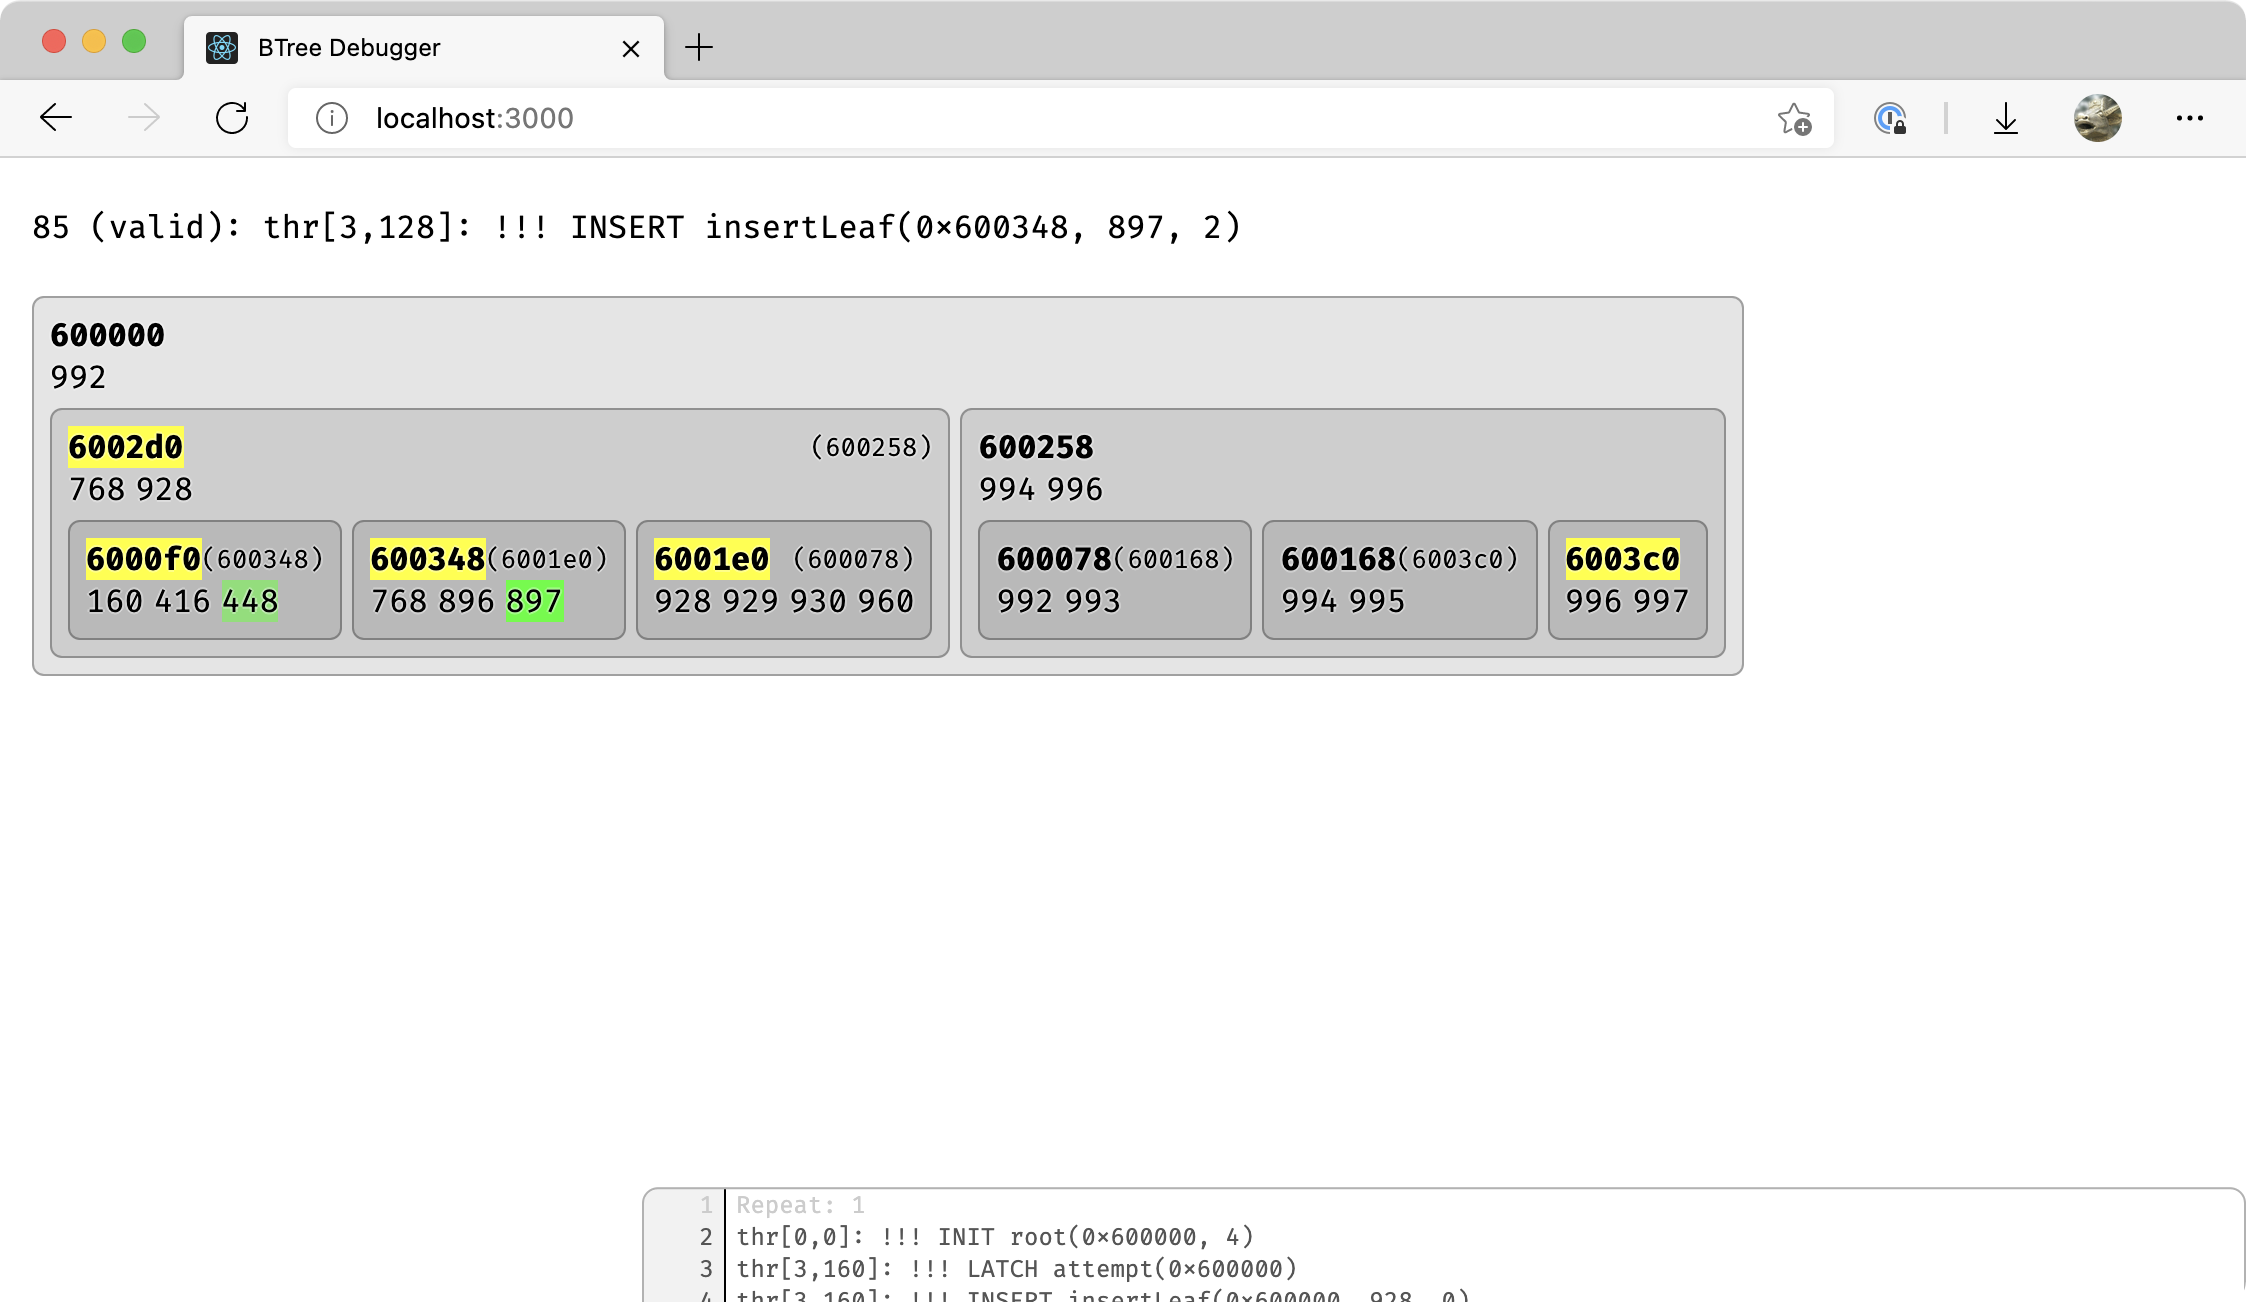
\includegraphics[width=\textwidth]{components/figure/debugger.png}
  \caption{Web based visual debugger displaying the internal state of a tree. Red boxes denote split nodes not yet inserted to the parent node. A highlighted node address indicate that a thread has latched that node.}
  \label{figure:debugger}
\end{figure}

In the case of multiple B-Tree variants, to avoid duplicating tests and ensure the correctness of both implementations, typed tests are used to repeat the same logic over a list of types \cite{gtest-advanced}, as seen in \cref{lst:gtest-typed}. The \code{typename} of each class will be available as a static field within \code{TestFixture} itself.

\begin{listing}
  \begin{minted}{cpp}
template <typename C> class TestSuite : public testing::Test {
public:
  using Implementation = C;
};

using TypeList = ::testing::Types<A, B>;
TYPED_TEST_SUITE(TestSuite, TypeList);

TYPED_TEST(TestSuite, Test) {
  typename TestFixture::Implementation impl;
  // ... rest of test implementation
}
    \end{minted}
  \caption{Snippet of a GoogleTest typed test}\label{lst:gtest-typed}
\end{listing}